\documentclass{report}

\usepackage[utf8]{inputenc}
\usepackage[T1]{fontenc}
\usepackage[francais]{babel}
\usepackage{textcomp}
\usepackage{amssymb}
\usepackage{algorithm}
\usepackage{algorithmic}
\usepackage{lipsum}
\usepackage{listingsutf8}
\usepackage{xcolor}
\usepackage[top=2.5cm,bottom=2.5cm,right=2.5cm,left=2.5cm]{geometry}
\usepackage{graphicx}

\lstset
    {language=C,
    frame=L,
    xleftmargin=\parindent,
    columns=flexible,
    basicstyle=\ttfamily\small,
    inputencoding=utf8/latin1,
    breaklines=true,
    breakautoindent=true,
    keywordstyle=\color{blue},
    stringstyle=\color{orange},
    commentstyle=\itshape\color{green!20!black},
    tabsize=2,
    extendedchars=true,
    showspaces=false,
    showstringspaces=false,
    numbers=left,
    numberstyle=\tiny,}

\newenvironment{myindentpar}[1]%
    {\begin{list}{}%
             {\setlength{\leftmargin}{#1}}%
             \item[]%
     }
     {\end{list}}


\title{Compte rendu du TP1 de Structure de Données}
\author{\textsc{Laurent} Valentin, \textsc{Malrin} Vincent}

\begin{document}

\maketitle

\tableofcontents

\setcounter{chapter}{1}
\newpage
\section{Objet du TP}\label{objet}
Création d'un agenda grâce à une liste chaînée à deux niveaux.

\section{Structure de données}\label{sdd}
Chaque bloc du premier niveau contient une année,
le numéro de la semaine, un pointeur vers la liste des actions de la semaine et un pointeur vers la semaine suivante.
Les blocs du second niveau (liste chainée des actions) contiennent le jour de la semaine, l'heure, 
le nom de l'action et le pointeur vers l'action suivante.

\begin{small}
\begin{verbatim}

       --        ---------------
 p_sem|  |----->| chaine_sem[7] |
       --        ---------------        ----------------
                | action_s      |----->| chaine_act[14] |
                 ---------------        ----------------        ----------------
                | suiv          |      | suiv           |----->| chaine_act     |
                 ---------------        ----------------        ----------------
                        |                                      | suiv           |
                        |                                       ----------------
                        \/
                 ---------------
                | chaine_sem    |
                 ---------------        ----------------
                | action_s      |----->| chaine_act     |
                 ---------------        ----------------
                | suiv          |      | suiv           |
                 ---------------        ----------------

\end{verbatim}
\end{small}

\newpage
\section{Organisation du code source}\label{source}
\subsubsection{agenda.h}
C'est le fichier d'entête.

\subsubsection{insertion.c}
Ce fichier contient les fonctions :
\begin{myindentpar}{2cm}
\begin{itemize}
    \item InsererSem
    \item InsererAct
    \item Liberation
\end{itemize}
\end{myindentpar}

\subsubsection{recherche.c}
Ce fichier contient les fonctions :
\begin{myindentpar}{2cm}
\begin{itemize}
    \item RechercheSem
    \item RechercheAct
\end{itemize}
\end{myindentpar}

\subsubsection{suppression.c}
Ce fichier contient les fonctions :
\begin{myindentpar}{2cm}
\begin{itemize}
    \item SuppressionAct
    \item SuppressionSem
\end{itemize}
\end{myindentpar}

\subsubsection{afficher.c}
Ce fichier contient les fonctions :
\begin{myindentpar}{2cm}
\begin{itemize}
    \item Affichage
    \item Menu
\end{itemize}
\end{myindentpar}

\subsubsection{bilatere.c}
Ce fichier contient les fonctions :
\begin{myindentpar}{2cm}
\begin{itemize}
    \item TransfoBilatere
    \item IsertionBil
    \item LiberationBil
\end{itemize}
\end{myindentpar}

\subsubsection{ecriture.c}
Ce fichier contient les fonctions :
\begin{myindentpar}{2cm}
\begin{itemize}
    \item Ecriture
    \item Lecture
\end{itemize}
\end{myindentpar}

\subsubsection{recherche\_motif.c}
Ce fichier contient les fonctions :
\begin{myindentpar}{2cm}
\begin{itemize}
    \item RechercheMotif
    \item AffichageMotif
\end{itemize}
\end{myindentpar}

\newpage
\section{Codes Sources}\label{codes}
\subsection{EN TÊTE : agenda.h}
\begin{small}
\lstinputlisting{../agenda.h}

\newpage
\subsection{MAIN : agenda.c}
\lstinputlisting{../agenda.c}

\subsection{INSERTION : insertion.c}
\lstinputlisting{../insertion.c}

\subsection{AFFICHAGE : afficher.c}
\lstinputlisting{../afficher.c}

\subsection{RECHERCHE : recherche.c}
\lstinputlisting{../recherche.c}

\subsection{SUPPRESSION : suppression.c}
\lstinputlisting{../suppression.c}

\subsection{RECHERCHE DE MOTIF : motif.c}
\lstinputlisting{../motif.c}

\subsection{ECRITURE : ecriture.c}
\lstinputlisting{../ecriture.c}

\subsection{BILATÈRE : bilatere.c}
\lstinputlisting{../bilatere.c}

\newpage
\subsection{MAKEFILE}
\lstinputlisting[language=make]{../makefile}
\end{small}


\newpage
\section{Jeux de tests}
\subsection{Cas à tester}
\subsubsection{Lecture et Insertion (Question 1)}
Cas à tester :
\begin{myindentpar}{2cm}
\begin{itemize}
    \item Cas de fichier non valide (pour la lecture)
    \item Cas liste vide
    \item Cas cellule unique
    \item Cas général (10 cellules)
\end{itemize}
\end{myindentpar}

\subsubsection{Recherche et Suppression (Question 3)}
Cas à tester :
\begin{myindentpar}{2cm}
\begin{itemize}
    \item Cas liste vide
    \item Cas cellule unique
    \item Cas général (10 cellules)
    \begin{itemize}
        \item Recherche en début
        \item Recherche au milieu
        \item Recherche en fin
    \end{itemize}
    \item Tests sur des dates non valides
\end{itemize}
\end{myindentpar}

\subsubsection{Recherche de Motif (Question 2)}
Cas à tester :
\begin{myindentpar}{2cm}
\begin{itemize}
    \item Cas liste vide
    \item Cas général (10 cellules)
    \begin{itemize}
        \item Recherche en début
        \item Recherche au milieu
        \item Recherche en fin
    \end{itemize}
    \item Test sur un motif non valide
    \item Test sur un motif multiple
\end{itemize}
\end{myindentpar}

\subsubsection{Ecriture (Question 2)}
Cas à tester :
\begin{myindentpar}{2cm}
\begin{itemize}
    \item Cas liste vide
    \item Cas général (10 cellules)
\end{itemize}
\end{myindentpar}

\subsubsection{Liste Bilatère (Question 4)}
Cas à tester :
\begin{myindentpar}{2cm}
\begin{itemize}
    \item Cas liste vide
    \item Cas cellule unique
    \item Cas général (3 cellules, pour facilité l'affichage sur DDD)
\end{itemize}
\end{myindentpar}

\newpage
\subsection{Fichiers en entrée}

\subsubsection{Test de listes vides : donnee0.txt}
\lstinputlisting{../donnee0.txt}

\subsubsection{Test de cellule unique : donnee1.txt}
\lstinputlisting{../donnee1.txt}

\subsubsection{Test du cas général (10 cellules) : donnee10.txt}
\lstinputlisting{../donnee10.txt}

\subsubsection{Test du cas général (4 cellules) : donnee4.txt}
\lstinputlisting{../donnee4.txt}

\subsubsection{Fichier d'écriture : donnee\_e.txt}

\newpage
\subsection{Execution}
\subsubsection{Lecture et Insertion (Question 1)}
\begin{itemize}
    \item Cas Fichier invalide : \./agenda 1 fichier\_innexistant.txt
\vspace{0.5cm}
\lstinputlisting{../tests/tests_insert1.txt}
\vspace{0.5cm}

    \item Cas liste vide : \./agenda 1 donnee0.txt
\vspace{0.5cm}
\lstinputlisting{../tests/tests_insert2.txt}
\vspace{0.5cm}

    \item Cas liste unique : \./agenda 1 donnee1.txt
\vspace{0.5cm}
\lstinputlisting{../tests/tests_insert3.txt}
\vspace{0.5cm}

    \item Cas général : \./agenda 1 donnee10.txt
\vspace{0.5cm}
\lstinputlisting{../tests/tests_insert4.txt}
\end{itemize}

\newpage
\subsubsection{Recherche (Question 3)}
\begin{itemize}

    \item Recherche -> Cas liste vide : \./agenda 2 donnee0.txt 201342108
\vspace{0.5cm}
\lstinputlisting{../tests/tests_rech1.txt}
\vspace{0.5cm}

    \item Recherche -> Cas cellule unique : \./agenda 2 donnee1.txt 201342108
\vspace{0.5cm}
\lstinputlisting{../tests/tests_rech2.txt}
\vspace{0.5cm}

    \item Cas général (recherche au début) : \./agenda 2 donnee10.txt 201342108 (libelle : Calcul)
\vspace{0.5cm}
\lstinputlisting{../tests/tests_rech3.txt}
\vspace{0.5cm}

    \item Cas général (recherche au milieu) : \./agenda 2 donnee10.txt 201343210 (libelle : Systeme)
\vspace{0.5cm}
\lstinputlisting{../tests/tests_rech4.txt}
\vspace{0.5cm}

    \item Cas général (recherche au fin) : \./agenda 2 donnee10.txt 201403517 (libelle : Liberte)
\vspace{0.5cm}
\lstinputlisting{../tests/tests_rech5.txt}
\vspace{0.5cm}

    \item Cas général (date incorrecte) : \./agenda 2 donnee10.txt 201343209
\vspace{0.5cm}
\lstinputlisting{../tests/tests_rech6.txt}
\end{itemize}

\newpage
\subsubsection{Suppression (Question 3)}
\begin{itemize}

    \item Suppression -> Cas liste vide : \./agenda 3 donnee0.txt 201342108
\vspace{0.5cm}
\lstinputlisting{../tests/tests_supp1.txt}
\vspace{0.5cm}

    \item Suppression -> Cas cellule unique : \./agenda 3 donnee1.txt 201342108
\vspace{0.5cm}
\lstinputlisting{../tests/tests_supp2.txt}
\vspace{0.5cm}

    \item Cas général (Suppression au début) : \./agenda 3 donnee10.txt 201343108 (libelle : Calcul)
\vspace{0.5cm}
\lstinputlisting{../tests/tests_supp3.txt}
\vspace{0.5cm}

    \item Cas général (Suppression au milieu) : \./agenda 3 donnee10.txt 201343208 (libelle : TP de SDD)
\vspace{0.5cm}
\lstinputlisting{../tests/tests_supp4.txt}
\vspace{0.5cm}

    \item Cas général (Suppression au fin) : \./agenda 3 donnee10.txt 201403517 (libelle : Liberte)
\vspace{0.5cm}
\lstinputlisting{../tests/tests_supp5.txt}
\vspace{0.5cm}

    \item Cas général (date incorrecte) : \./agenda 3 donnee10.txt 201343209
\vspace{0.5cm}
\lstinputlisting{../tests/tests_supp6.txt}
\end{itemize}

\newpage
\subsubsection{Ecriture (Question 2)}
\begin{itemize}
    \item Cas liste vide : \./agenda 4 donnee0.txt donnee\_e0.txt
\vspace{0.5cm}
\lstinputlisting{../tests/tests_ecr1.txt}
\vspace{0.5cm}

Affichage de fichier donnee\_e0.txt
\vspace{0.5cm}
\lstinputlisting{../donnee_e0.txt}
\vspace{0.5cm}

    \item Cas général : \./agenda 4 donnee10.txt donnee\_e1.txt
\vspace{0.5cm}
\lstinputlisting{../tests/tests_ecr2.txt}
\vspace{0.5cm}

Affichage du fichier donnee\_e1.txt :
\vspace{0.5cm}
\lstinputlisting{../donnee_e1.txt}
\end{itemize}

\newpage
\subsubsection{Bilatere (Question 4)}
\begin{itemize}
    \item Cas liste vide : \./agenda 5 donnee0.txt

\vspace{0.5cm}
\lstinputlisting{../tests/tests_bil1.txt}
\vspace{0.5cm}

Après l'execution de la fonction TransfoBilatere on a sur DDD :
\begin{figure}[!h] 
    \begin{center}
    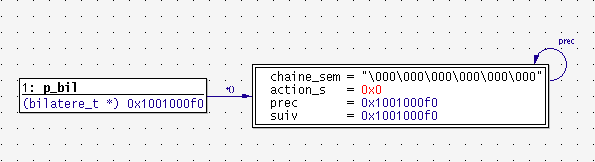
\includegraphics[width=15cm]{liste_vide.png}
    \caption{Cas liste vide} %la légende
    \end{center}
\end{figure}
\end{itemize}

\newpage
\begin{itemize}
    \item Cas cellule unique : \./agenda 5 donnee1.txt

\vspace{0.5cm}
\lstinputlisting{../tests/tests_bil2.txt}
\vspace{0.5cm}

Après l'execution de la fonction TransfoBilatere on a sur DDD :
\begin{figure}[!h] 
    \begin{center}
    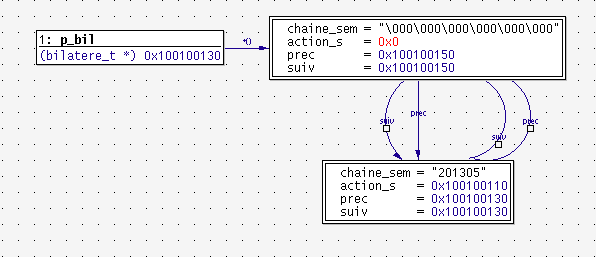
\includegraphics[width=15cm]{cas_unique.png}
    \caption{Cas liste vide} %la légende
    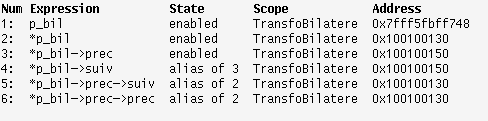
\includegraphics[width=15cm]{tab_cas_unique.png}
    \end{center}
\end{figure}
\end{itemize}

\newpage
\begin{itemize}
    \item Cas général (4 cellules): \./agenda 5 donnee4.txt

\vspace{0.5cm}
\lstinputlisting{../tests/tests_bil3.txt}
\vspace{0.5cm}

Après l'execution de la fonction TransfoBilatere on a sur DDD :
\begin{figure}[!h] 
    \begin{center}
    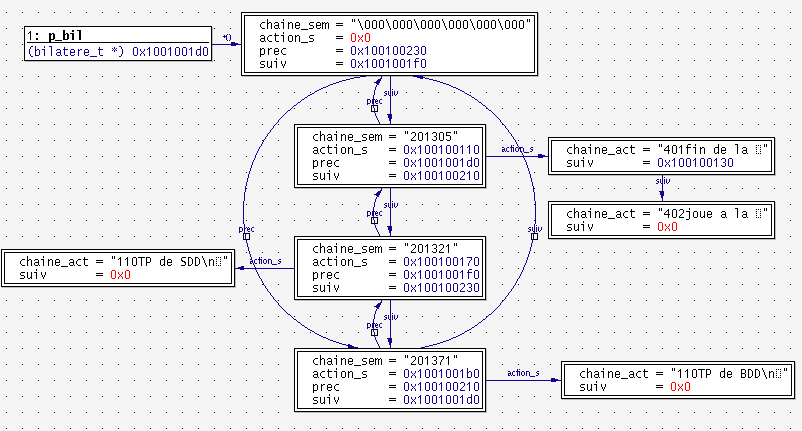
\includegraphics[width=18cm]{cas_general.png}
    \caption{Cas liste vide} %la légende
    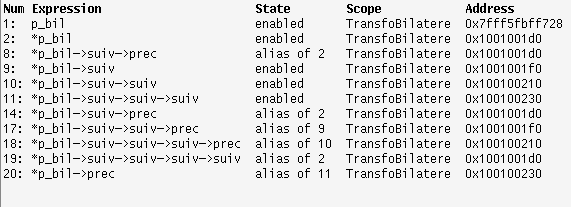
\includegraphics[width=15cm]{tab_cas_general.png}
    \end{center}
\end{figure}
\end{itemize}

\newpage
\subsubsection{Recherche Motif (Question 2)}
\begin{itemize}
    \item Cas liste vide : \./agenda 6 donnee0.txt SDD
\vspace{0.5cm}
\vspace{0.5cm}
\lstinputlisting{../tests/tests_motif1.txt}
\vspace{0.5cm}
\vspace{0.5cm}

    \item Cas général (recherche en début) : \./agenda 6 donnee10.txt Calcul
\vspace{0.5cm}
\lstinputlisting{../tests/tests_motif2.txt}
\vspace{0.5cm}

    \item Cas général (recherche au milieu) : \./agenda 6 donnee10.txt SDD
\vspace{0.5cm}
\lstinputlisting{../tests/tests_motif3.txt}
\vspace{0.5cm}

    \item Cas général (recherche en fin) : \./agenda 6 donnee10.txt Liberte
\vspace{0.5cm}
\lstinputlisting{../tests/tests_motif4.txt}
\vspace{0.5cm}

    \item Cas général et libelle innexistant : \./agenda 6 donnee10.txt truc
\vspace{0.5cm}
\lstinputlisting{../tests/tests_motif5.txt}
\vspace{0.5cm}

    \item Cas général et libelle multiple : \./agenda 6 donnee10.txt TP
\vspace{0.5cm}
\lstinputlisting{../tests/tests_motif6.txt}
\vspace{0.5cm}

\end{itemize}

\end{document}
